%\begin{itemize}
%    \item
%        Weshalb wurde das benutzte mathematische Modell gew\"ahlt?
%    \item
%        Weshalb wird ein Schaltregler benutzt?
%    \item
%        Weshalb wurde ein eigenes PCB entwickelt statt ein Steckbrett verwendet?
%    \item
%        Wie soll unser Ger\"at bedient werden k\"onnen?
%\end{itemize}

This section primarily deals with the underlying mathematics used to model the
various  configurations  of  solar  cells  the device  needs  to  be  able  to
emulate. Additionally, it presents a brief overview of the hardware.

% **************************************************************************** %
\subsection{The Model}
% **************************************************************************** %

The aim in developing  our model was to find the  sweet spot between usability
and  accuracy. It  should  have  a  small,  comprehensive  set  of  parameters
which  can be  easily understood  by the  user, while  still representing  the
actual physics  accurately enough to  yield good results.


% **************************************************************************** %
\subsubsection{Single Solar Cell}
% **************************************************************************** %

\begin{minipage}{0.6\textwidth}
    The single diode model of the ideal PV cell\cite{ref:villa:pvmodel} serves
    as  a basis  for our  model.   The I-V  characteristic of  this model  can
    be  expressed  with equation  \ref{eq:I-V_old},  whereby  $I_{pv}$ is  the
    generated current,  $I_o$ is the diode  current and $ V_T$  is the thermal
    voltage.
\end{minipage}
\begin{minipage}{0.4\textwidth}
    \begin{equation} \label{eq:I-V_old}
        I = I_{pv} - I_o \left[ \exp \left( \frac{V}{V_T} \right) - 1 \right]
    \end{equation}
\end{minipage}

\begin{minipage}{0.7\textwidth}
    Although these  three parameters depend  on the junction  temperature, the
    inclusion  of the  junction  temperature  into our  model  as a  parameter
    would  only  contribute a  minor  correction  factor, negligible  for  our
    purposes.  For this reason we can simplify our model if we assume that the
    temperature is equal to the nominal temperature $T_n = 298.15K$.

    The  thermal  voltage  is  defined  in  equation  \ref{eq:thermalvoltage},
    whereby $T$ is the junction temperature, $k$ is the Boltzman constant, $q$
    is  the elementary  charge and  $a$ is  the diode  ideality factor,  which
    typically  lies around  1.2  for silicon  substrates. This  gives us  $V_T
    \approx 30.8mV$ for one cell.

    The  current generated  by the  cell is  calcualted according  to equation
    \ref{eq:cellcurrent}, whereby $I_n$  is the nominal current  and $G$ and
    $G_n$ is the actual and nominal solar irradiation, respectively.

    A  common optimisation,  according to\cite{ref:villa:pvmodel},  is to  set
    $I_n \approx  I_{sc}$ and  again assume that  the temperature  is constant
    ($T  =  T_n$),   giving  us  $\Delta_T  =  0$   and  simplifying  equation
    \ref{eq:cellcurrent} to equation \ref{eq:I_pv}.

    Finally, the diode  leakage current at the nominal  temperature (for other
    temperatures  please  see  \cite{ref:villa:pvmodel})  is  calculated  with
    equation \ref{eq:I_o}.

    If  we  insert  equations  \eqref{eq:I_o} and  \eqref{eq:I_pv}  back  into
    \eqref{eq:I-V_old} we get equation \ref{eq:IAlmostDone}.

    If   we  now   assume  $V_{oc}   >   5  \cdot   V_T$  we   can  say   that
    $e^{\frac{V_{oc}}{V_T}}-1  \approx e^{\frac{V_{oc}}{V_T}}$  and our  final
    formula becomes equation \eqref{eq:I-V}.
\end{minipage}
\begin{minipage}{0.3\textwidth}
    \begin{equation} \label{eq:thermalvoltage}
        V_T = a k T / q
    \end{equation}
    \begin{equation} \label{eq:cellcurrent}
        I_{pv} = \left( I_n + K_I \Delta_T \right) \frac{G}{G_n}
    \end{equation}
    \begin{equation} \label{eq:I_pv}
        I_{pv} = I_{sc} \frac{G}{G_n}
    \end{equation}
    \begin{equation} \label{eq:I_o}
        I_o = \frac{I_{sc}}{e^{V_{oc} / V_T} - 1}
    \end{equation}
    \begin{equation} \label{eq:IAlmostDone}
        I = I_{sc} \left( \frac{G}{G_n} - \frac{e^{\frac{V}{V_T}}-1}{e^{\frac{V_{oc}}{V_T}}-1} \right)
    \end{equation}
    \begin{equation} \label{eq:I-V}
        I = I_{sc} \left( \frac{G}{G_n} - e^{\frac{V - V_{oc}}{V_T}} \right)
    \end{equation}
\end{minipage}



% **************************************************************************** %
\subsubsection{Multiple Cells in Series}
% **************************************************************************** %

If the solar irradiation is the same  for  every  cell in series, then the whole
array  can be simulated using equation \eqref{eq:I-V}, where $V_{oc}$  and  $V_T$
are linearly scaled with the number of cells.

If the irradiation is not the same for all  cells,  such  as  when  one  cell  is
shaded, a more complex model must be used.

\begin{minipage}{0.5\textwidth}
    \center
    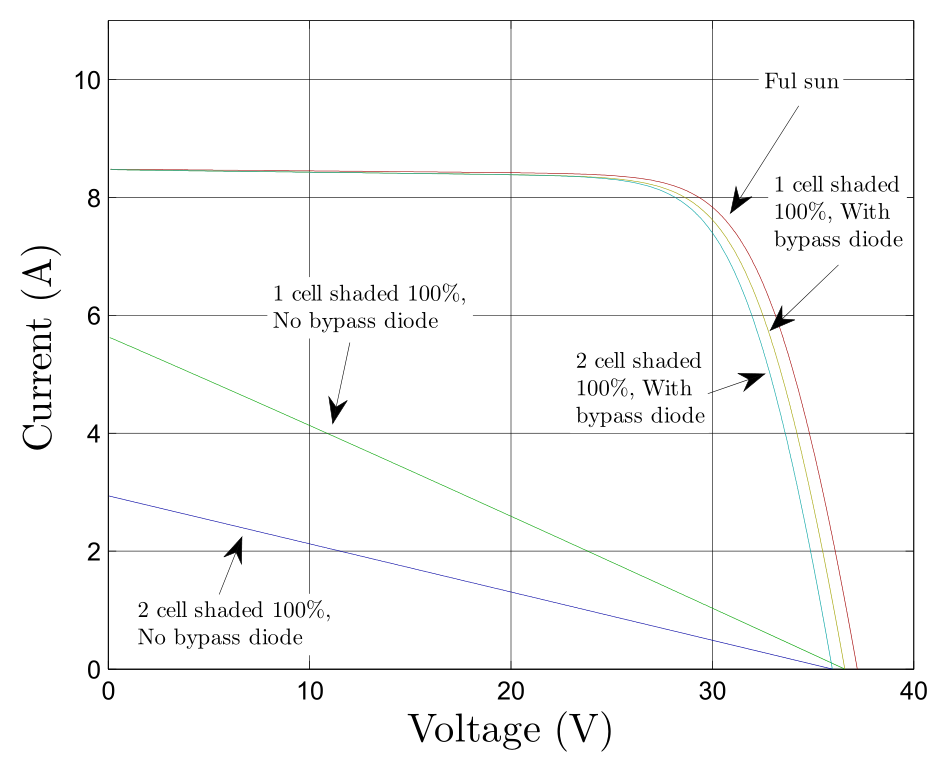
\includegraphics[width=\textwidth]{images/model/shaded.png}
    \captionof{figure}{I-V curves for different configurations and shaded cells\cite{ref:tian:model}}
    \label{fig:model:shaded}
\end{minipage}
\begin{minipage}{0.5\textwidth}
	\center
    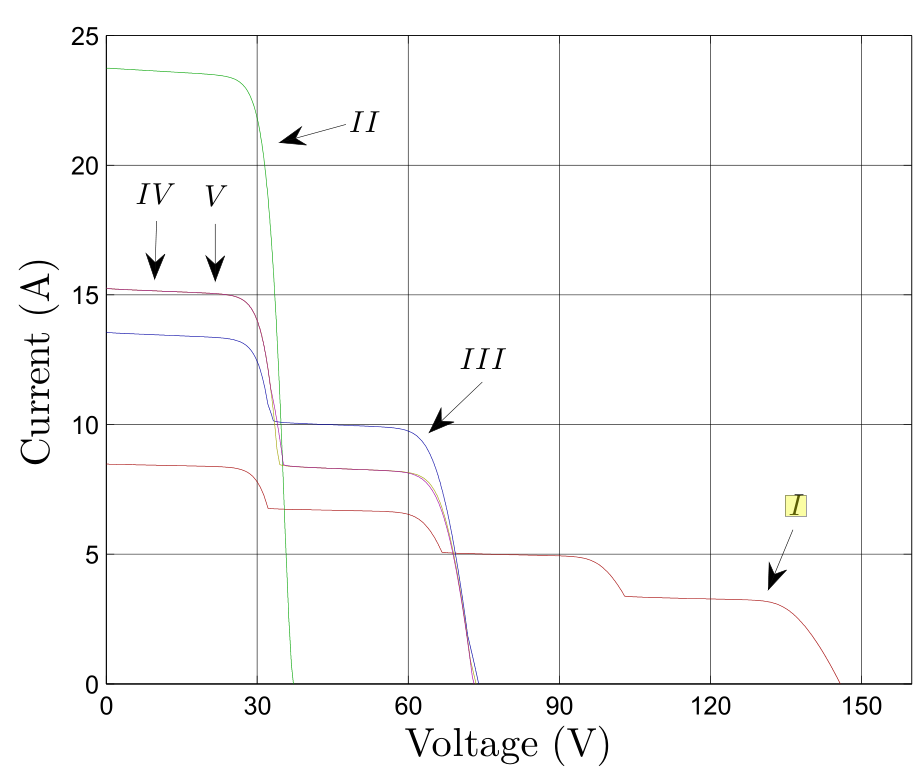
\includegraphics[width=\textwidth]{images/model/steps.png}
    \captionof{figure}{The typical characteristic of modules connected in series or in parallel}
    \label{fig:model:steps}
\end{minipage}


Figure \ref{fig:model:shaded} shows various  characteristic curves of a shaded
PV  module and  the effect  of bypass  diodes on  them.  In  our model  we can
emulate the I-V  curve of an array with  a shaded cell and no  bypass diode by
setting $V_T = V_{oc}$.

%Figure \ref{fig:model:shaded}  shows  what  varied  characteristics  of a shaded
%PV-module  look  like  and  how  bypass  diodes affect them. In our model we can
%imitate  the  I-V  curve of an array with a shaded cell and no bypass  diode  by
%setting $V_T = V_{oc}$.

The  characteristic  curves shown  in  Figure  \ref{fig:model:steps} show  how
``steps'' emerge when  two or more modules with bypass  diodes, which are each
exposed  to different  irradiation  intensities, are  connected in  series. To
emulate  this behaviour,  we take  a number  of curves  with decreasing  short
circuit current and increasing open  circuit voltage and determine which curve
is applicable by checking what curve returns the maximum current for the given
voltage.


% **************************************************************************** %
\subsection{Implementation of Regulation}
\label{subsec:regimplementation}
% **************************************************************************** %

To increase  accuracy in emulating  the I-V characteristic curve,  both output
voltage and output current of the  device's operating point are monitored.  If
the  operating  point  is  above  the  $-\frac{\SI{1}{\volt}}{\SI{1}{\ampere}}
=  \SI{-1}{\ohm}$ slope  (``A''  in figure  \ref{fig:controlcircuit:vicurve}),
more  accurate  regulation can  be  achieved  by  operating the  regulator  in
constant  current  mode.   In  contrast,  if  the  operating  point  is  below
the  \SI{-1}{\ohm} slope  (``B'' in  figure \ref{fig:controlcircuit:vicurve}),
operating the  regulator in constant voltage  mode will yield a  more accurate
result.

A       more        detailed       explanation       can        be       found
in      section       \ref{subsec:iv-curve-operating-points}      on      page
\pageref{subsec:iv-curve-operating-points}.

\begin{minipage}{0.5\textwidth}
    \center
    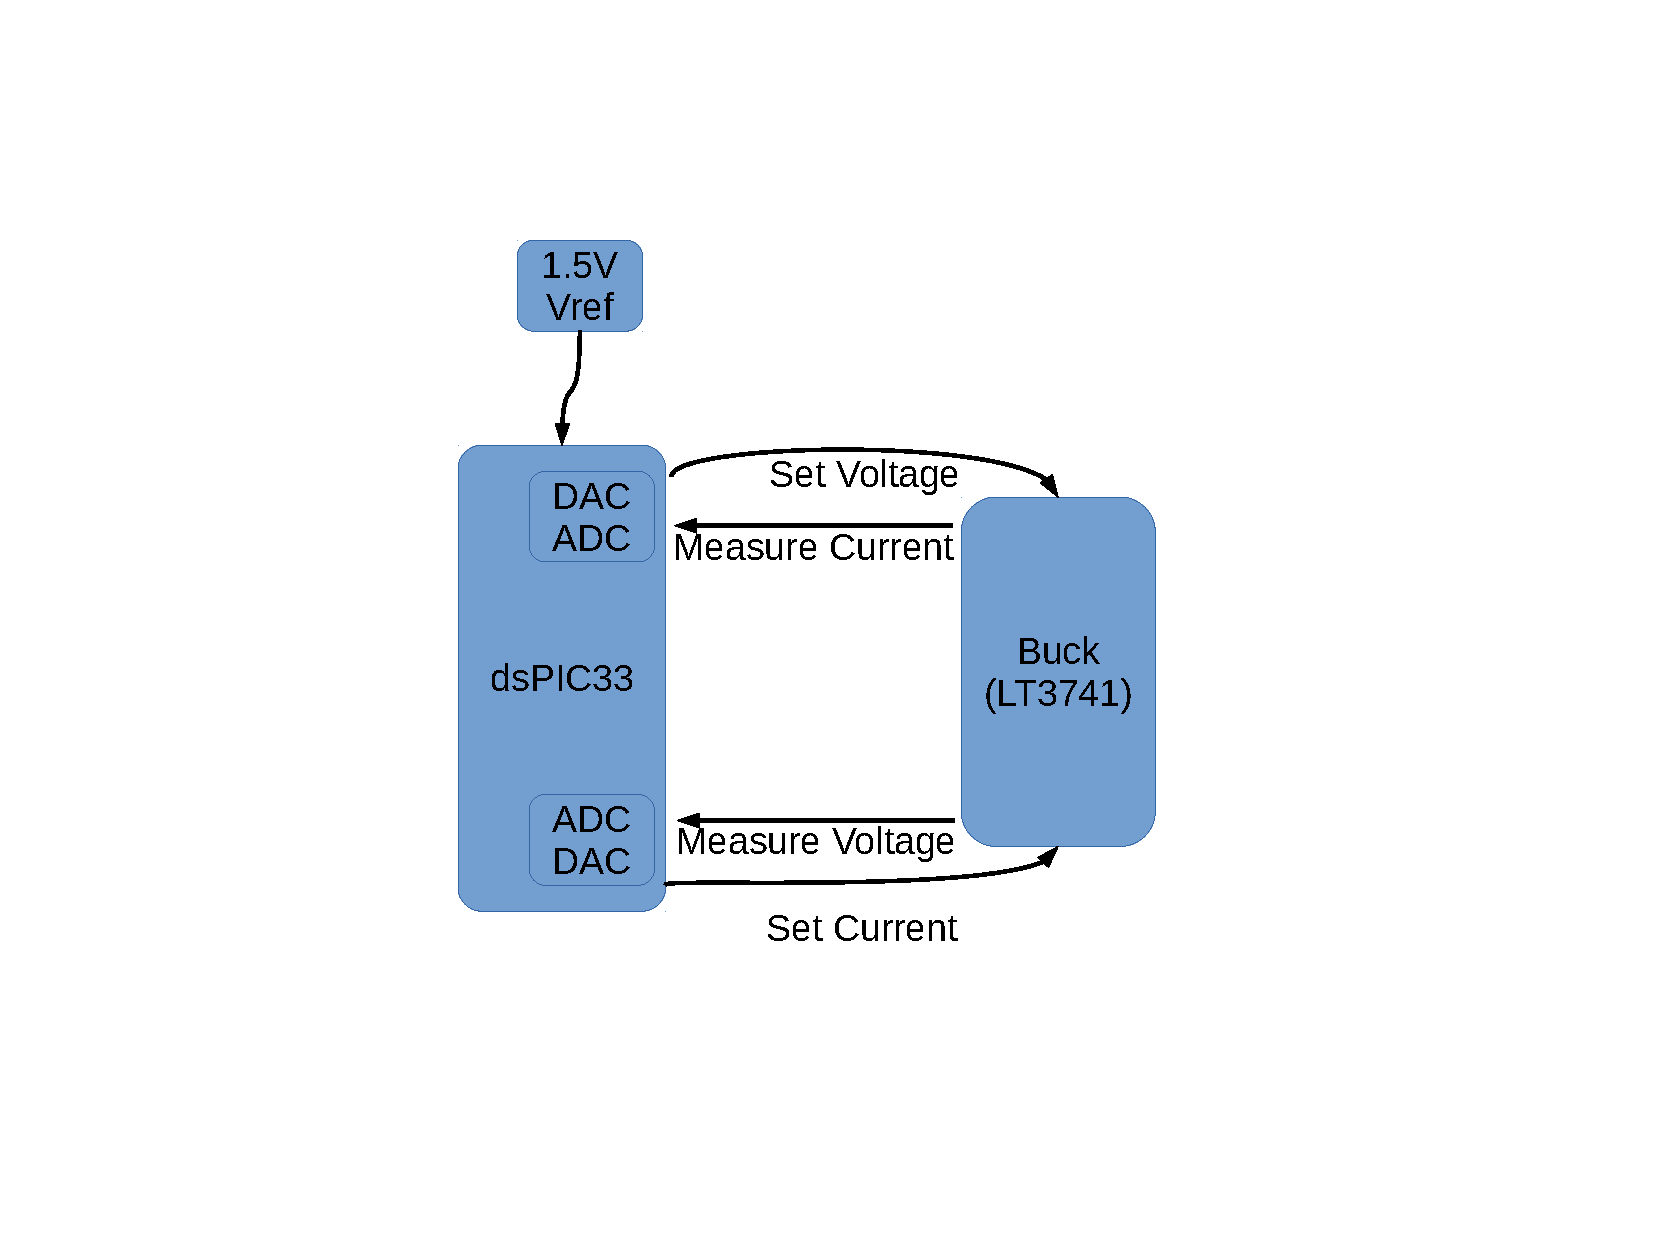
\includegraphics[width=\textwidth,trim=140 140 120 100,clip]{images/block-diag-control.pdf}
    \captionof{figure}{Block diagram of control circuit}
    \label{fig:controlcircuit:schcematic}
\end{minipage}
\begin{minipage}{0.5\textwidth}
    \center
    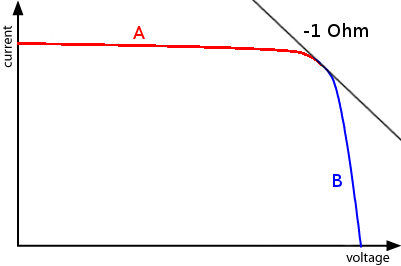
\includegraphics[width=\textwidth]{images/vi-curve.png}
    \captionof{figure}{I-V-Curve with \SI{-1}{\ohm} slope indicated}
    \label{fig:controlcircuit:vicurve}
\end{minipage}


% **************************************************************************** %
\subsection{Hardware}
% **************************************************************************** %

Our device is based  on a microcontroller, which is used  to handle user input
and output and  controls the step-down converter.  Power  delivery is realised
with a  prebuilt DC  power supply  unit. In addition  to interacting  with the
device directly, users can also connect a PC to our device by USB and then use
our front-end  software \emph{Smooth}  to interface  with the  device (section
\ref{subsec:frontend}, p. \pageref{subsec:frontend}ff).

With  an  eye  towards  potential  serial production,  we  developed  our  own
PCB. This  allows tight  control over  impedances in  the connections  between
critical  components  and   brings  the  behavior  of   the  prototype  device
much  closer   to  a  mass   produced  version  than  a   breadboard  solution
could. This  is because  trace  routing lengths  and  component placement  are
crucial  factors,  as  is  discussed  in  section  \ref{sec:verification}  (p.
\pageref{sec:verification}ff), \emph{Verification}.
